% This is based on the LLNCS.DEM the demonstration file of
% the LaTeX macro package from Springer-Verlag
% for Lecture Notes in Computer Science,
% version 2.4 for LaTeX2e as of 16. April 2010
%
% See http://www.springer.com/computer/lncs/lncs+authors?SGWID=0-40209-0-0-0
% for the full guidelines.
%

\documentclass[12pt,a4paper]{article}
\usepackage{graphicx}
\usepackage[usenames, dvipsnames]{color}
\usepackage{todonotes}  % Can add notes on margins. To disable type \usepackage[disable]{todonotes}

\begin{document}

\title{Our Project}

\author{Tor Dj\"{a}rv\inst{1} \and Noam Gavrielov\inst{2}\and Luca Riz\inst{3}}

          % typeset the title of the contribution

\begin{abstract}
\dots
\end{abstract}
%
\section{NushellX} \label{NushellX}
%
%
In this part we present the results we obtained using NushellX \cite{nush} and comment on them. We focus  on the $sd$-shell, specifically on oxygen isotopes and their properties. In the first subsection we analyze the spectra of oxygen isotopes and the capability of different interactions (i.e. new-usd family of interactions \cite{usd} (USDA and USDB) and coupled cluster effective interaction \cite{ccei} (CCEI)) to reproduce spectra. The second subsection is devoted to the study of Fermi and Gamow-Teller $\beta$-decay of $^{22}$O and how the USDB and CCEI interactions fulfill sum rules.

\subsection{Oxygen isotopes spectra with different interactions} \label{Oxygen}
%
We analyze how the different interactions reproduce the excitation energy of the first $2^+$ state in even-even oxygen isotopes from $^{18}$O to $^{26}$O and compare to experiment. This is seen in Figure \ref{fig:2+/0+} \todo[linecolor=black,backgroundcolor=orange]{add error bars to figure?}  and gives an indication on the location of the shell closure. The latter  arises when the excitation energy from the g.s. to the first excited $2^+$ state is at maximum.

\begin{figure}[htb!]
\centering
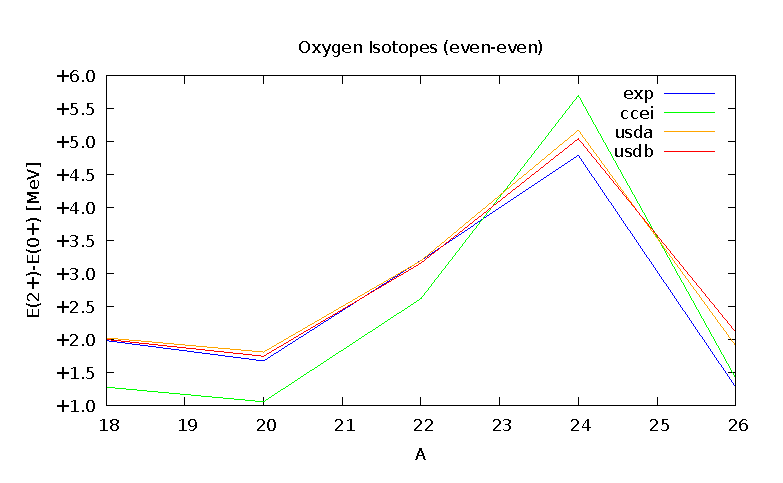
\includegraphics[width=0.8\textwidth]{2+_over_0+.eps}
\caption{Excitation energy of the first $2^+$ state in oxygen isotopes (even-even).}
\label{fig:2+/0+}
\end{figure}

The USDA and USDB interactions give similar results,  are in good agreement with experimental results and give a good description of the shell closure at $^{24}$O. Since USDB has more linear combination of parameters than USDA it generates a better agreement with the experimental results. 
The CCEI interaction underestimates the excitation energies up to $^{26}$ oxygen\todo[linecolor=black,backgroundcolor=orange]{why?}, while at shell closure it emphasize this effect by overestimating the first $2^+$ state energy\todo[linecolor=black,backgroundcolor=orange]{why?}. 
It is interesting to note that CCEI interactions seems to give a good description in rich neutron isotopes, close to the neutron drip line\todo[linecolor=black,backgroundcolor=orange]{why?}.

We next explore the spectra of even-odd oxygen isotopes. Among them we analyze the spectrum of $^{19}$O since it has the largest amount of experimental data. The results are shown in Figure \ref{fig:19O}. Note that the experimental results show also negative parity states (blue lines), which are not included in our theoretical calculations since we are working in the $sd$ model space. For completeness black dots in the experimental panel indicates states which have not been assigned to a definite parity.
\begin{figure}[htb!]
\centering
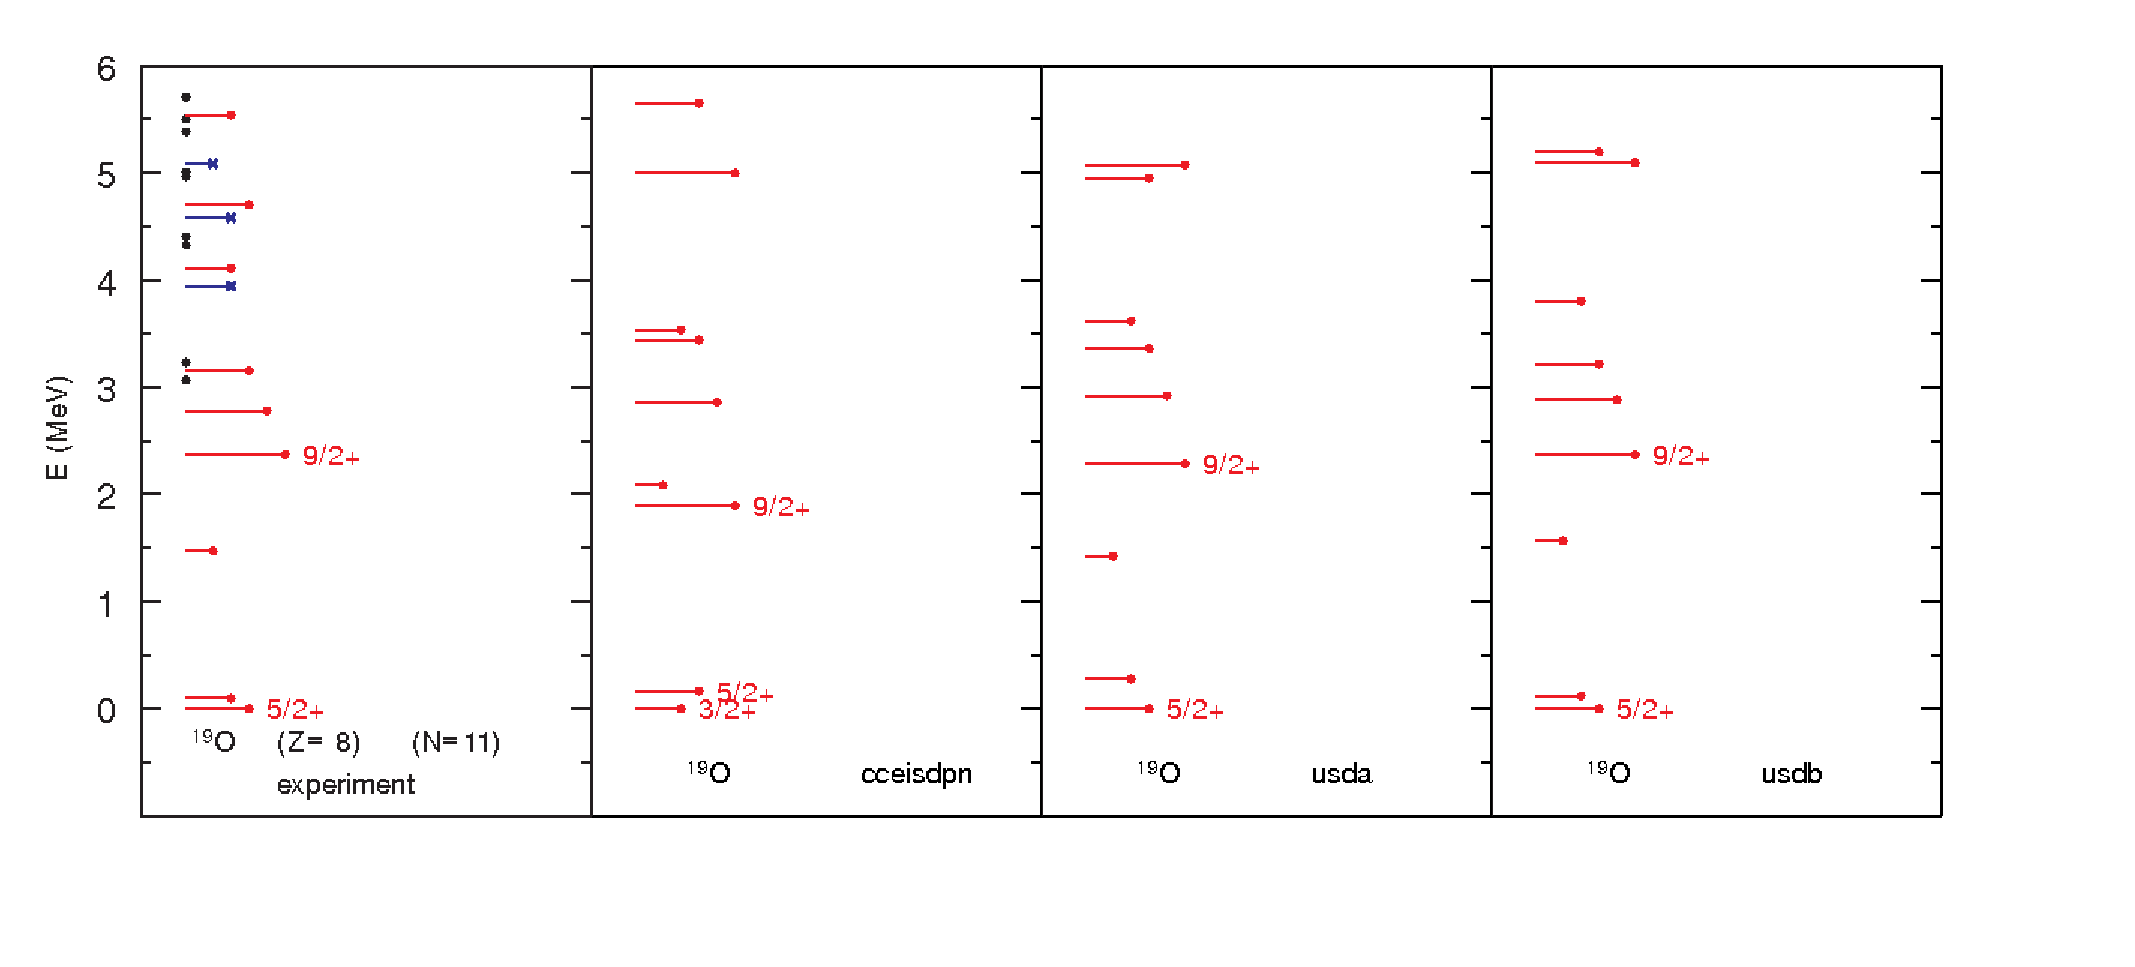
\includegraphics[width=\textwidth]{19O.eps}
\caption{$^{19}$O spectrum with different interactions compared to experiments.}
\label{fig:19O}
\end{figure}

The USDA and USDB reproduce the correct spin orderings, where the USDA yields better results up to the first $1/2^+$ at energy 1.422 MeV and the USDB yields better results from the first $9/2^+$ at energy 2.370 MeV up to the second $3/2^+$ at energy 3.802 MeV. The differences are not significant though and further tests for comparison could be electromagnetic transition rates.
The CCEI exchanges the order of the first $3/2^+$ with the g.s. and the order of the first $9/2^+$ and the first $1/2^+$, causing both pairs to be nearly degenerate. \todo[linecolor=black,backgroundcolor=orange]{I would try to explain why this occurs, if possible}The former case is reasonable since the g.s. and the first $3/2^+$ are nearly degenerate,  however the latter case exhibits a larger discrepancy from experiment.

%
\subsection{\textcolor{red}{(Spectroscopic Factors?)}}
\textcolor{red}{Not sure if we add also the part on spectroscopic factors \dots I think if I add also this part it becomes too long.} \textcolor{blue}{I agree (Noam)}. 
%

%
\subsection{Fermi and Gamow-Teller $\beta$-decay of $^{22}$O}
%
On top of energies, it is insightful to examine other observables in order to understand better the differences between different interactions. We analyze the $\beta$-decay of $^{22}$O to $^{22}$F.
We perform the calculations using NushellX for the USDB \todo[linecolor=black,backgroundcolor=orange]{What about USDA? If it is similar to USDB we should point that out.} and CCEI interactions. 
\begin{table}[h!]
\caption{Sum Rules}
\begin{center}
\begin{tabular}{l@{\qquad}l@{\qquad}r@{\qquad}rl}
\hline
\multicolumn{1}{l}{\rule{0pt}{12pt}
                   }&\multicolumn{1}{l}{\rule{0pt}{12pt} sum rule}&\multicolumn{1}{l}{CCEI}&\multicolumn{2}{l}{USDB}\\[2pt]
\hline\rule{0pt}{12pt}
sum b(f)            &  $N_i-Z_i=6$   & 5.9993 & 6.0000 &\\
sum qf$\cdot$b(gt)  &  $\ge 3\cdot(N_i-Z_i)=18$  & 6.0346 & 10.0335 &\\[2pt]
\hline
\end{tabular}
\end{center}
\end{table}

Both interactions fulfill the theoretical Fermi sum rule, but in different ways.
The contribution of the CCEI interaction to the Fermi sum rule b(f) splits among different states: this is because the e interaction has several nearly degenerate levels which mix. The USDB interaction gives all the contribution to b(f) in one single state, which is the isobar analogue of the $^{22}$O \textcolor{red}{(is this true? - Ch. 44 Brown's notes)}. 
\textcolor{red}{(Anyone has more to say about Gamow-Teller sum rule?)}

Let us compare the results obtained with the two different interactions to the experimental results for the q-value and the half-life. Note that one has to include more than only the default ten levels for each spin state in NushellX in order to get significant results, otherwise too much information is neglected.
\begin{table}[h!]
\caption{q-value and t$_{1/2}$}
\begin{center}
\begin{tabular}{r@{\qquad}r@{\qquad}r@{\qquad}r@{\qquad}l}
\hline
\multicolumn{1}{l}{\rule{0pt}{12pt}
                   }&\multicolumn{1}{l}{exp}&\multicolumn{1}{l}{CCEI}&\multicolumn{2}{l}{USDB}\\[2pt]
\hline\rule{0pt}{12pt}
q-value [MeV]   &     6.489 & 6.847 & 8.437 &\\
t$_{1/2}$ [sec] &     2.25  & 0.478 & 2.620 &\\[2pt]
\hline
\end{tabular}
\end{center}
\end{table}

The CCEI interaction gives a good description of the q-value, but underestimates the half-life, while the USDB interaction is in good agreement with the experimental value for the half-life, but slightly overestimates the q-value.

%
\paragraph{Notes and Comments}
\textcolor{red}{I think we should make the conclusions together.}

%
% ---- Bibliography ----
%
\begin{thebibliography}{3}
%
\bibitem {nush}
B. A. Brown and W. D. M. Rae, Nuclear Data Sheets 120, 115 (2014)
\bibitem {usd}
B. A. Brown and W. A. Richter, Physical Review C 74, 034315 (2006)
\bibitem {ccei}
G. R. Jansen, M. D. Schuster, A. Signoracci, G. Hagen and P. Navr\'atil, Physical Review C 94, 011301(R) (2016)

\end{thebibliography}

\appendix
\section{Noam}

\subsection{NushellX \ref{NushellX}} 
\begin{enumerate}
	\item Changed some words.
\end{enumerate}

\subsection{Oxygen isotopes spectra with different interactions \ref{Oxygen}}
\begin{enumerate}
	\item Rephrased some of the explanations and added some of mine with some questions.
	\item It seems as though there is a general behavior of the CCEI interaction in which pairs of levels in $^{19}$O are nearly degenerate - ($3/2^+$,$5/2^+$), ($9/2^+$,$1/2^+$) and ($5/2^+$,$3/2^+$). It would be interesting to understand why this occurs.
\end{enumerate}

\subsection{General Remarks}
\begin{enumerate}
	\item How should we merge our notes?
\end{enumerate}


\end{document}
